\Object{Tâche}
{
Une tâche représente un fil d'exécution, \textsl{i.e.} un ensemble d'instructions exécuté sur un même processeur. Elle peut s'exécuter (état \lstinline{ACTIVE}), attendre d'avoir la main sur le processeur (état \lstinline{ACTIVABLE}) ou attendre l'autorisation d'une ou plusieurs autres tâches. 

Si une des méthode \lstinline{attendre}, \lstinline{entrer}, \lstinline{suspendre}, ou \lstinline{prendre} est appelée, la tâche appelante passe dans le méta-état \lstinline{BLOQUE} jusqu'à ce que l'une des méthode suivante soit appelée : \lstinline{signaler}, \lstinline{sortir}, \lstinline{reprendre} ou \lstinline{donner}.
}
{
La structure \lstinline{struct tache} est composée de :
\begin{itemize}
	\item id : \lstinline{int}
	\item etat : \lstinline{enum \{ ACTIVABLE, ACTIVE, SUSPENDUE, ATTENTE\_EVENEMENT, ATTENTE\_REGION, ATTENTE\_SEMAPHORE \}} 
	\item attente\_id : \lstinline{int}
	\item evenements\_attente : Liste d'identifiants d'événements.
	\item priorite : \lstinline{int} 
\end{itemize}
}
{
Toutes les primitives avec un type de retour entier, renvoient -1 en cas d'erreur (\textsl{e.g} plus de mémoire disponible, identifiant invalide, \textsl{etc.}). Sauf indication contraire, elles renvoient 0 en cas de succès.

\begin{itemize}
	\item \lstinline{int demarrer(struct tache* t)} : Démarre la tâche passée en paramètre.
	\item \lstinline{int suspendre(struct tache* t)} : Suspend la tâche passée en paramètre. 
	\item \lstinline{int terminer(struct tache* t)} : Tue la tâche passée en paramètre.
	\item \lstinline{struct tache* tacheCourrante()} : Renvoie la structure de la tâche courante, \textsl{i.e.} la tâche d'où cette fonction est appelée.
\end{itemize}
}
{
\begin{figure} [htp]
\centering
%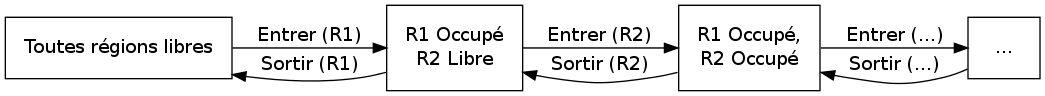
\includegraphics{img/etatTache.png}
\end{figure}
}
{L'ordonnancement des tâches est délégué à une agence.}
